\section{Auswertung}
\label{sec:Auswertung}

\subsection{Detektorscan}
Zunächst wird der Detektorscan analysiert. 
Dafür werden die Messwerte in \autoref{fig:Detektorscan} aufgetragen.
Die Intensität gibt dabei die Anzahl der gemessenen Photonen pro Zeiteinheit an, in diesem Teil des Versuchs pro Sekunde.
\begin{figure}
    \centering
    \caption{Die aufgenommenen Intensitätsmesswerte werden gegen den Winkel aufgetragen. Zudem wird eine Gauß-Verteilung an die Werte angepasst und daraus die Halbwertsbreite und das Intensitätsmaximum berechnet und makiert.}
    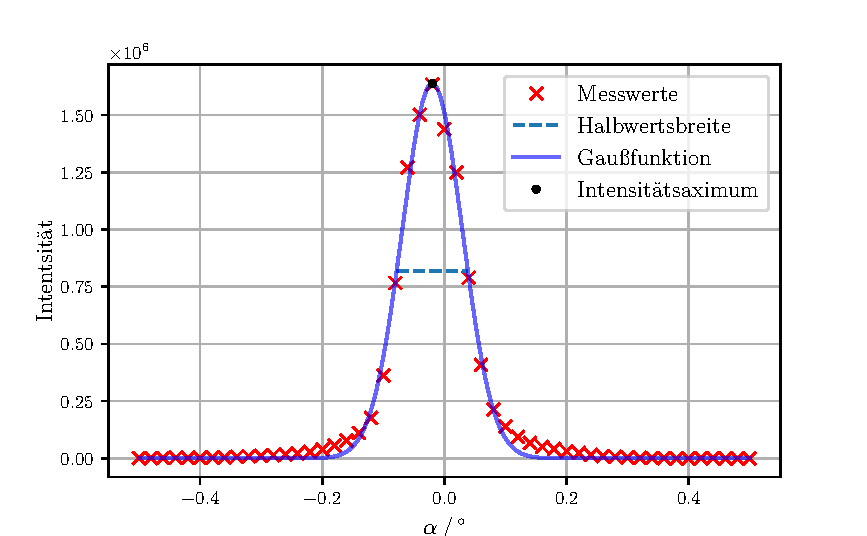
\includegraphics[width=0.75\textwidth]{content/data/Detectorscan.pdf}
    \label{fig:Detektorscan}
\end{figure}
An die Messwerte wird eine Gauß-Verteilung angepasst.
Dazu wird die Funktion \textit{curve\_fit} des python Pakets \textit{scipy} \cite{scipy} genutzt.
Dieses führt eine Ausgleichsrechung für die Funktion 
\begin{equation*}
    I(\alpha) = \frac{a}{\sqrt{2\pi\sigma^2}} \exp{\frac{-\left (\alpha- \mu \right)^2}{2\sigma^2}}
\end{equation*}
mit den Messwerten durch.
Die Ausgleichsrechung hat die Werte 
\begin{align*}
    a &= \SI{1637959.863}{\degree / \second}\\
    \sigma &= \SI{20.205}{\degree} \\
    \mu &= \SI{-0.019}{\degree}
\end{align*}
ergeben.
Die dadurch definierte Gauß-Verteilung ist ebenfalls in \autoref{fig:Detektorscan} zu sehen.
Aus dieser wird das Intensitätsmaxium $I_\text{max}$ und die Halbwertsbreite $FWHM$ bestimmt.
Die bestimmten Werte sind
\begin{align*}
    I_\text{max} &= \SI{1637959.685}{\per \second} \, , \\
    FWHM &= \SI{0.116}{\degree}.
\end{align*}
\FloatBarrier
\subsection{Z-Scan}
Die Messwerte des Z-Scans sind in \autoref{fig:zscan} zu sehen.
Da nicht alle Werte für die Auswertung relevant sind werden nur die Werte zwischen $z = -0.4$ bis $0.7 \, \si{\milli\meter}$ geplottet.
\begin{figure}
    \centering
    \caption{Die relevanten Messwerte des Z-Scans. Zudem wurden durch grüne Linien die Strahlbreite makiert.}
    \includegraphics[width=0.75\textwidth]{content/data/zscan.pdf}
    \label{fig:zscan}
\end{figure}
In der \autoref{fig:zscan} ist zudem die Strahlbreite $d_0$ in grün makiert.
Der Strahl hat eine Breite von 
\begin{align*}
    d_0 &= \SI{0.24}{\milli\meter}.
\end{align*}
\FloatBarrier
\subsection{Rockingscan}
Die Messwerte der Rockingscans sind in \autoref{fig:rockingscan} zu finden.
\begin{figure}
    \centering
    \caption{Die Messwerte des Rockingscans und die makierten Geometriewinkel.}
    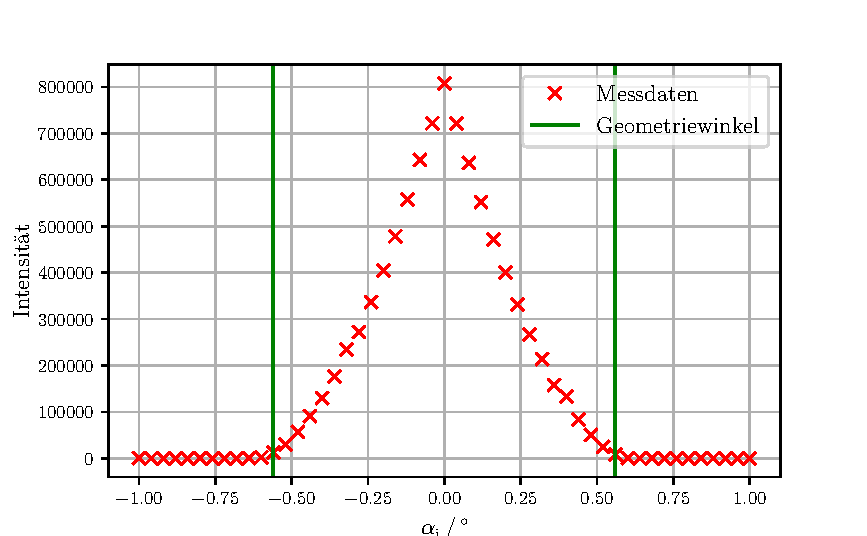
\includegraphics[width=0.75\textwidth]{content/data/rockingscan.pdf}
    \label{fig:rockingscan}
\end{figure}
In grün sind in der \autoref{fig:rockingscan} die Geometriewinkel $\alpha_\text{g}$ makiert.
Zudem wird aus dem Geometriewinkel links und rechts der Mittelwert $\bar{\alpha_\text{g}}$ gebildet.
Die Geometriewinkel haben einen Wert von 
\begin{align*}
    \alpha_\text{g, links} &= \SI{-0.560}{\degree} \\
    \alpha_\text{g, rechts} &= \SI{0.560}{\degree} \\
    \bar{\alpha_\text{g}} &= \SI{0.560}{\degree}.
\end{align*}
Aus der Strahlbreite und der Länge der Probe $D=\SI{20}{\milli\meter}$ ist es zudem möglich den theoretischen Geometriewinkel zu berechnen.
Dies geschieht mit Gleichung \eqref{eq:geometriewinkel}.
Der daraus resultierende theoretische Geometriewinkel beträgt
\begin{align*}
    \alpha_\text{g, theo} &= \SI{0.687}{\degree}.
\end{align*}
\FloatBarrier
\subsection{Reflektivitätsmessung}
Für die Reflektivitätsmessung wird ein diffuser Scan und eine direkter Scan durchgeführt.
Die dabei aufgenommenen Intensitäten werden durch die maximale Intensität geteilt, die zuvor durch den Detektorscan bestimmt wird.
Dabei wir die maximale Intensität mit fünf multipliziert, da sich die Integrationszeit der beiden Messungen um Faktor fünf unterscheiden.
Dies ergibt die Gleichung 
\begin{equation*}
    R = \frac{I}{5\cdot I_\text{max}}
\end{equation*} 
zur Bestimmung der Reflektivität.
Die so bestimmten Reflektivitäten werden in \autoref{fig:reflek} gegen den Winkel $\alpha_\text{i}$ aufgetragen.
Sie werden vor der Darstellung im Plot durch 10 geteilt um im selben Wertebreich wie die anderen Funktionen zu liegen.
Zudem werden die bestimmten Reflektivitäten voneinander abgezogen um Rückstreueffekte zu eliminieren.
Die so entstandene Reflektivität ist in grün in \autoref{fig:reflek} zu sehen.
\\
Nun werden diese Werte mit dem Geometriefaktor $G$ korrigiert.
Dieser wird aus Gleichung \eqref{eqn:geometriefaktor}, für jeden Winkel $\alpha_\text{i}$ bestimmt.
Die zur Berechnung nötige Strahlbreite, Länge der Probe $D$ und Geometriewinkel $\alpha_\text{g}$ werden in den zuvor getätigten Scans bestimmt.
Die korrigierte Reflektivität ist in \autoref{fig:reflek} in braun dargestellt.
\\\\
Die Minima der korrigiert Reflektivität werden in \autoref{fig:reflek} mit roten Kreuzen markiert.
Die Minima werden mit der Funktion \textit{find\_peaks} aus dem python Paket \textit{scipy} \cite{scipy} bestimmt.
Aus den Abständen dieser wird die Schichtdicke $d$ berechnet.
Dafür wird der Abstand der Minima gemittelt um $\Delta \bar{x} _\text{minima}$ zu erhalten, woraus dann nach Gleichung
\begin{equation*}
    d = \frac{\lambda}{2\Delta \bar{x} _\text{minima}}
\end{equation*}
die Schichtdicke $d$ berechnet wird.
Dabei ist $\lambda = \SI{0.154}{\nano\meter}$ die Wellenlänge der im Versuch genutzten Strahlung.
Die so bestimmte Schichtdicke hat einen Wert von
\begin{align*}
    d = \SI{87.7(023)}{\nano\meter}.
\end{align*}

Zur alternativen Bestimmung der Schichtdicke kann der Parratt-Algorithmus genutzt werden.
Dieser wird in \autoref{sec:theorie} beschrieben.
Im Fall des Versuchs müssen drei Schichten beachtet werden.
Die des Silizium auf dem die Probe, also die Polystyrolschicht liegt, als unterste Schicht $N=3$.
Die Polystyrolschicht als zweite Schicht $N=2$ und die Luft als oberste Schicht $N=1$.
Alle unbekannten Parameter des Algorithmus werden nun abgeschätzt und so gut wie es geht an die, durch den Geometriefaktor korrigierte Reflektivität angepasst.
Die bekannten Werte sind $\delta_\text{1, luft} = 0$, die Position der ersten Grenzschicht $z_1= \SI{0}{\milli\meter}$ und die Wellenlänge der Strahlung $\lambda =\SI{0.154}{\nano\meter}$.
Der Wert $\delta_\text{i}$ lässt sich dabei aus dem Brechungsindex der Schicht mit der Gleichung
\begin{equation}
    \delta_\text{i} = 1- n_\text{i}
\end{equation}
berechnen.
Die Werte $\sigma_\text{i}$ entsprechen der Rauigkeit der jeweiligen Schicht.
Die manuell angepassten Werte ergeben sich zu:
\begin{align*}
    \delta_2 &= 0.5\cdot10^{-6}        \\ 
    \delta_3 &= 6.2\cdot10^{-6}        \\ 
    \sigma_1 &= \SI{0.85}{\nano\meter} \\ 
    \sigma_2 &= \SI{0.55}{\nano\meter} \\ 
    z_2 &= \SI{86.3}{\nano\meter}
\end{align*}
Die Theoriekurve mit den manuell angepassten Werten des Parratt-Algorithmus ist in \autoref{fig:reflek} als viollete Funktion zu finden.
Aus den Werten $\delta_2$ und $\delta_3$ wird anschließend der kritsiche Winkel $\alpha_\text{c}$ der beiden Schichten, mithilfe von Gleichung \eqref{eqn:kritisch_exp} bestimmt.
Die beiden kritsichen Winkel sind 
\begin{align*}
    \alpha_\text{c, PS} &= \SI{0.057}{\degree}\\
    \alpha_\text{c, Si} &= \SI{0.201}{\degree}.
\end{align*}
\\\\
Mit der Gleichung für die Fresnelreflektivität \eqref{eqn:fresnelreflektivitaet} wird eine ideale Reflektivität von Silizium bestimmt.
Der dafür benötigte kritische Winkel von Silizium $\alpha_\text{i, Si} = \SI{0.22}{\degree}$ wird dabei aus Quelle \cite[8]{alte_anleitung} entnommen.
Die so bestimmten ideale Fresnelreflektivität für Silizium wird in \autoref{fig:reflek} in rot gezeigt.
\\\\
\begin{figure}
    \centering
    \caption{Die aufgenommenen Messwerte die in die Reflektivitäten der Scans umgerechnet werden. Zudem die Theoriekurve aus dem Parratt-Algorithmus und aus der Fresnelreflektivität.
    Außerdem die Differenz der Reflektivität aus den Scans und die daraus berechnete korrigierte Reflektivität, von der die Minima der Oszillation makiert werden.}
    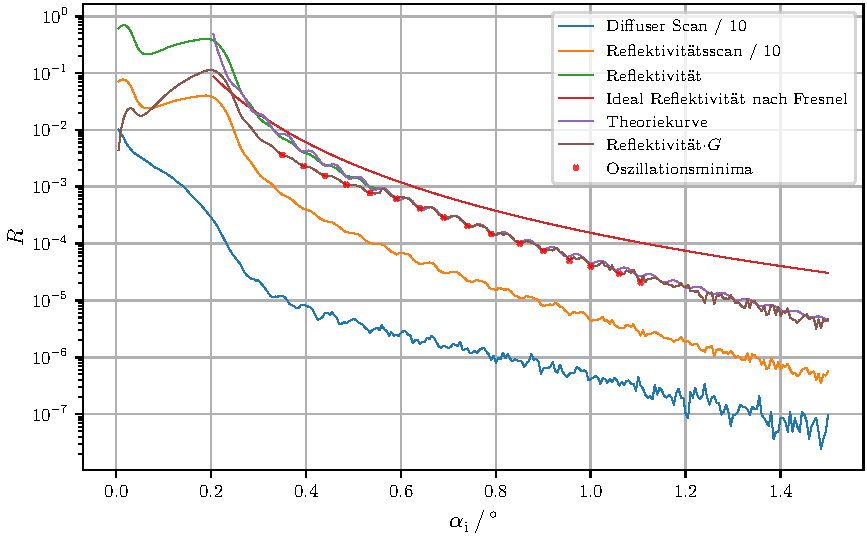
\includegraphics[width=0.75\textwidth]{content/data/reflek.pdf}
    \label{fig:reflek}
\end{figure}
\FloatBarrier